\section{实验结果及数据分析}

本章节将展示本次实验结果和数据分析,包括系统运行测试、创建表测试、新增数据测试、查询数据测试、删除数据测试。

\subsection{系统运行测试}

系统运行测试包括各个服务端节点的启动和停止、与系统状态的检测。首先通过如下命令启动各个节点,命令中通过命令行参数指定了每个节点的端口,并告知每个节点其余各个节点的域名和端口:

\begin{lstlisting}[language=bash]
python app.py --port 8000 --host-ports 127.0.0.1:8000 127.0.0.1:8001 127.0.0.1:8002
python app.py --port 8001 --host-ports 127.0.0.1:8000 127.0.0.1:8001 127.0.0.1:8002
python app.py --port 8002 --host-ports 127.0.0.1:8000 127.0.0.1:8001 127.0.0.1:8002
\end{lstlisting}

\begin{figure}[H]
    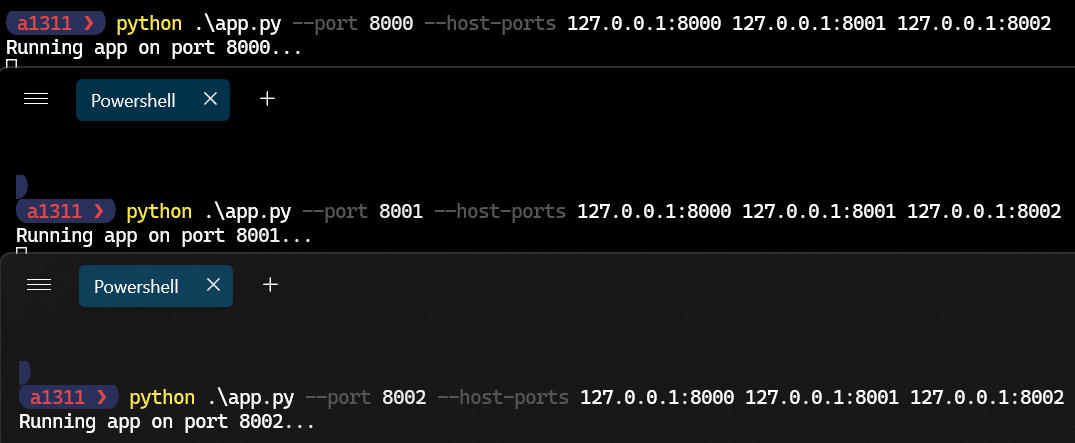
\includegraphics[width=\textwidth]{examples/各节点启动.png}
    \centering
    \caption{启动各个节点}
    \label{fig:test-start}
\end{figure}

如图\ref{fig:test-start}所示,各个节点提示成功信息。需要注意的是,这里是在本地进行测试的,故各个节点的域名都是127.0.0.1,本系统同样也支持在外部网络中运行。

之后,通过如下命令访问客户端,并于服务端连接:

\begin{lstlisting}[language=bash]
python client.py --host 127.0.0.1 --port 8000
\end{lstlisting}

\begin{figure}[H]
    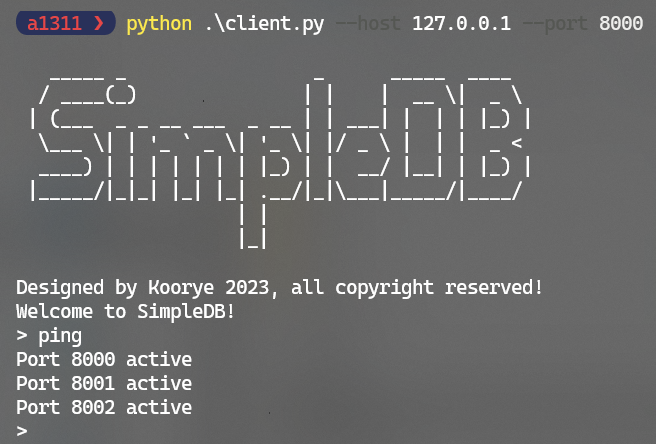
\includegraphics[width=0.7\textwidth]{examples/状态检测.png}
    \centering
    \caption{客户端连接}
    \label{fig:test-client}
\end{figure}

如图\ref{fig:test-client}所示,客户端成功连接,并通过本系统中提供的ping命令进行检测,结果是各个节点都在正常工作。

\begin{figure}[H]
    \centering
    \subfloat[]{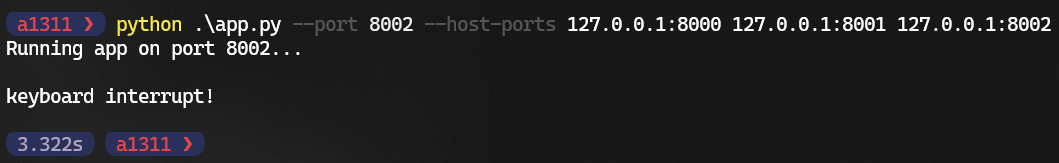
\includegraphics[width=1.0\textwidth]{examples/结束某个节点.png}} \\
    \subfloat[]{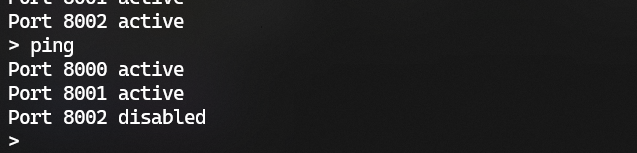
\includegraphics[width=1.0\textwidth]{examples/状态检测2.png}}
    \caption{ping命令演示}
    \label{fig:test-client2}
\end{figure}

倘若停止某个节点,其结果如图\ref{fig:test-client2}所示。可以看到,本系统成功检测出端口为8002的节点已停止运行。

\subsection{创建表测试}

本系统支持表格的创建与垂直划分,将根据表名的hash值将表格分配到不同的节点上进行持久化。此外,本系统基于Python进行开发,故实现了动态的字段类型。即各个字段无需手动分配类型,而是根据插入数据自动指定。因此,本系统可以通过如下SQL语句创建表格:

\begin{lstlisting}[language=sql]
create table <table_name> (
    <field1>,
    <field2>,
    <field3>,
    ...
);
\end{lstlisting}

需要注意的是,本系统仅实现了基础的表格创建功能,不支持主键、外键、自增等复杂功能。为了测试创建表格功能,在客户端中分别执行了创建用户表、图书表的命令。

\begin{figure}[H]
    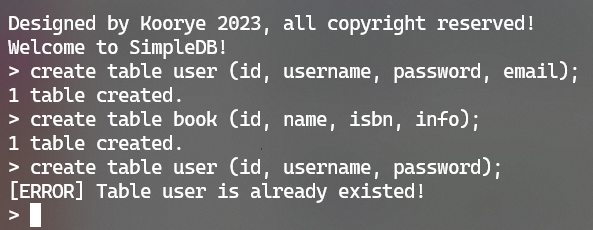
\includegraphics[width=0.6\textwidth]{examples/创建表.png}
    \centering
    \caption{创建表测试}
    \label{fig:test-create}
\end{figure}

如图\ref{fig:test-create}所示,user表和book表都被成功创建,之后再次创建user表时,则提示"Table user is already existed!"错误。

\begin{figure}[H]
    \subfloat[8000节点输出]{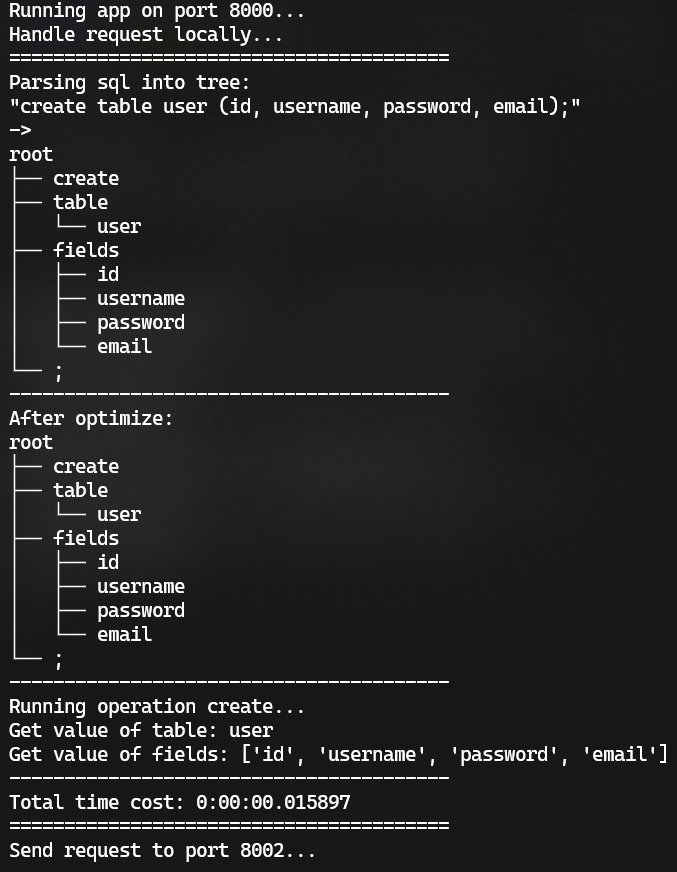
\includegraphics[width=0.44\textwidth]{examples/创建表-日志8000.png}}
    \subfloat[8002节点输出]{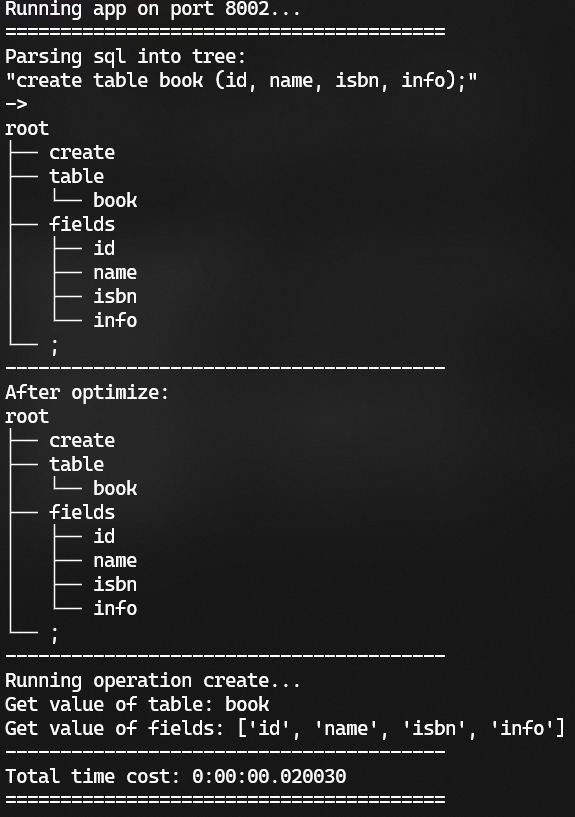
\includegraphics[width=0.395\textwidth]{examples/创建表-日志8002.png}}
    \centering
    \caption{创建表测试的屏幕输出}
    \label{fig:test-create-log}
\end{figure}

图\ref{fig:test-create-log}中展示了服务端终端的输出,由于客户端连接的端口为8000,因此节点8000直接接收客户端请求。之后,该节点会通过哈希策略分配请求所属的节点。这里节点8000就将user表视为本地请求,book表视为外部请求,并转发给8002节点。之后,各个节点都将请求通过语法解析、优化、执行等一系列流程,并于本地文件系统交互完成了创建表的目的。

\begin{figure}[H]
    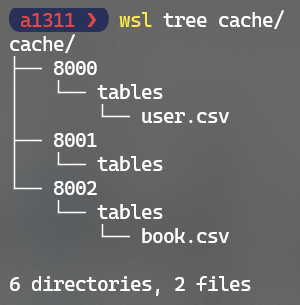
\includegraphics[width=0.4\textwidth]{examples/目录.png}
    \centering
    \caption{目录结构}
    \label{fig:dir}
\end{figure}

完成表创建命令后,目录结构如图\ref{fig:dir}所示,可以看到,各个表被存放在不同节点指定的目录内。需要注意的是,这里是本地运行模式,如果是多机运行,各个表将不会被存放在同一机器上,也就无法使用tree命令展示。

\subsection{新增数据测试}

在完成表创建后,就可以往表中插入数据了。插入数据的SQL命令格式如下:

\begin{lstlisting}[language=sql]
insert into <table_name>
    (<field1>, <field2>, ...)
values
    (<values1>, <value2>, ...);
\end{lstlisting}

\begin{figure}[H]
    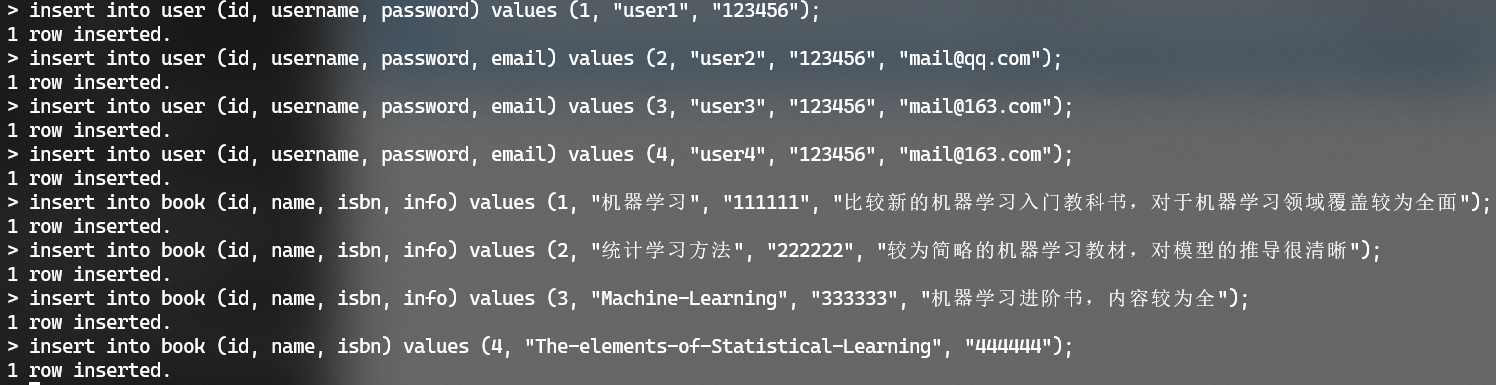
\includegraphics[width=\textwidth]{examples/插入数据.png}
    \centering
    \caption{新增数据}
    \label{fig:insert}
\end{figure}

图\ref{fig:insert}展示了客户端新增数据的结果,可以看出本系统支持不定类型和仅部分字段的数据插入方式,并支持中文等UTF-8字符编码。这里分别为user表和book表插入4条数据。

\begin{figure}[H]
    \subfloat[8000节点输出]{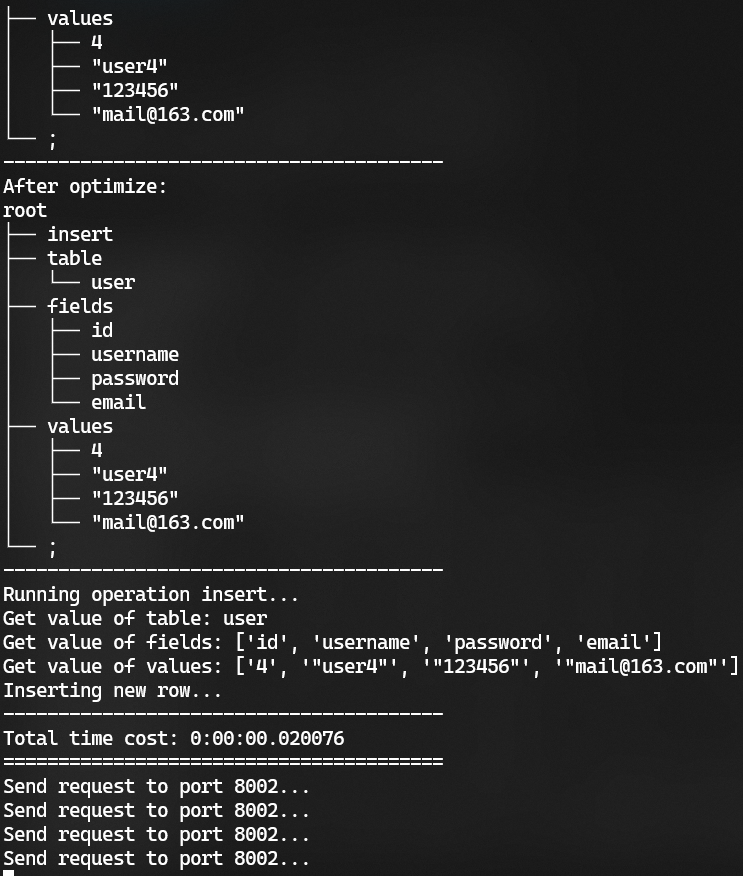
\includegraphics[width=0.4\textwidth]{examples/插入数据-8000.png}}
    \subfloat[8002节点输出]{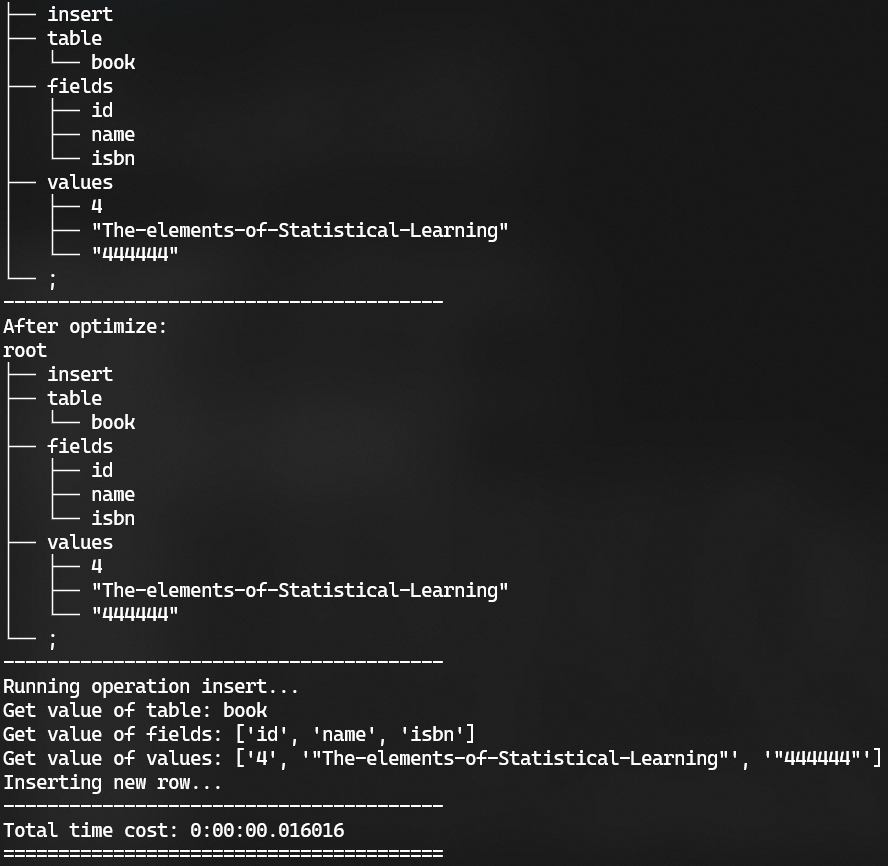
\includegraphics[width=0.5\textwidth]{examples/插入数据-8002.png}}
    \centering
    \caption{新增数据的屏幕输出}
    \label{fig:insert-log}
\end{figure}

图\ref{fig:insert-log}展示了服务端终端的输出,由于输出过长,这里仅能展示部分内容。可以看出,insert命令根据表名被转发,user表的请求被8000本地处理,book表的请求则被转发到8002进行处理。

\subsection{查询数据测试}

在查询数据之后,就可以进行查询。本系统实现了无条件的查询和带where的查询,不过不支持嵌套、级联等复杂查询逻辑。查询指令的格式如下:

\begin{lstlisting}[language=sql]
select
    (<field1>, <field2>, ...)
from
    <table>
[where <condition>];
\end{lstlisting}

\begin{figure}[H]
    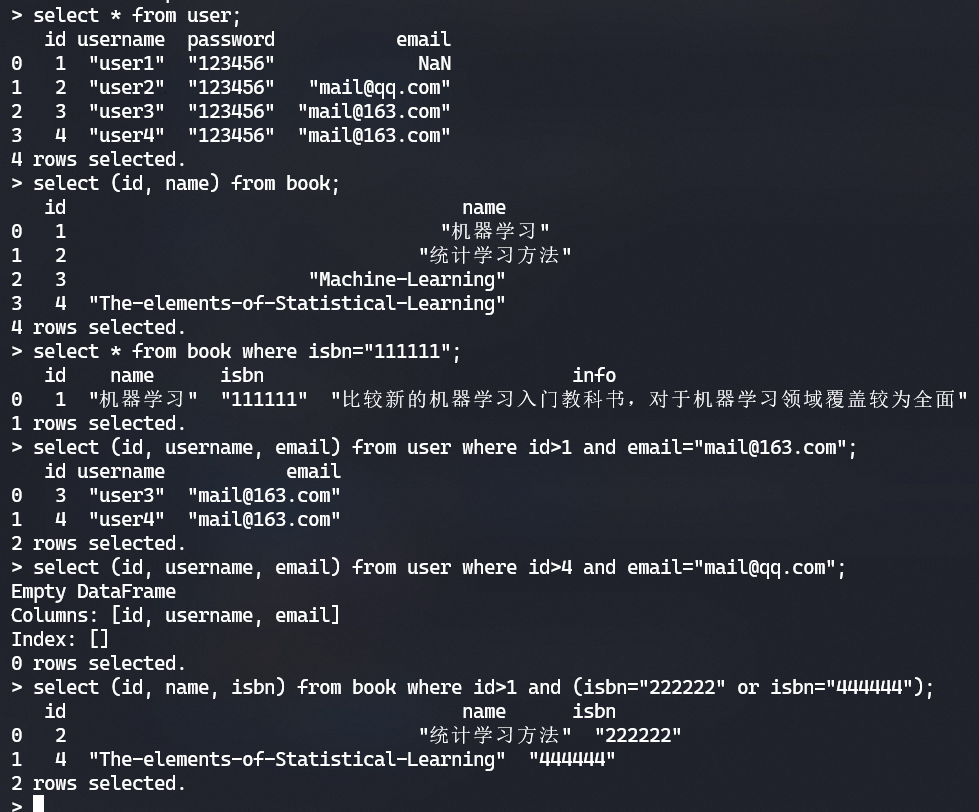
\includegraphics[width=\textwidth]{examples/查询.png}
    \centering
    \caption{查询数据}
    \label{fig:select}
\end{figure}

图\ref{fig:select}展示了在客户端输入查询语句的结果。可以看出,本系统支持多样化的查询语句,如指定列名进行查询,或使用*号代指全部列名。对于where子句,本系统也支持单一条件和多个条件,并通过逻辑运算符and/or进行连接,还支持通过括号运算符定义多个逻辑运算符之间的运算次序(括号可以多层嵌套)。例如,可以指定id>1且isbn为"222222"或isbn"333333"这样的复杂嵌套指令。

\begin{figure}[H]
    \subfloat[8000节点输出]{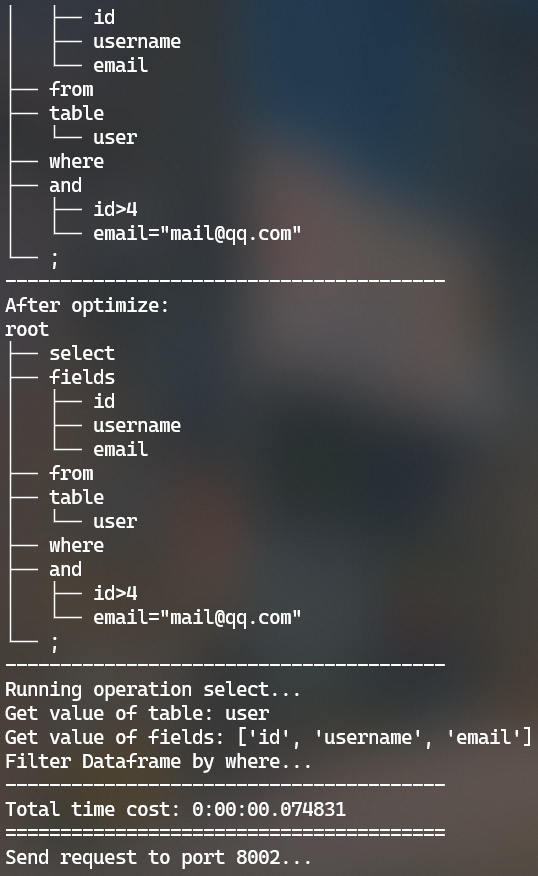
\includegraphics[width=0.525\textwidth]{examples/查询-8000.png}}
    \subfloat[8002节点输出]{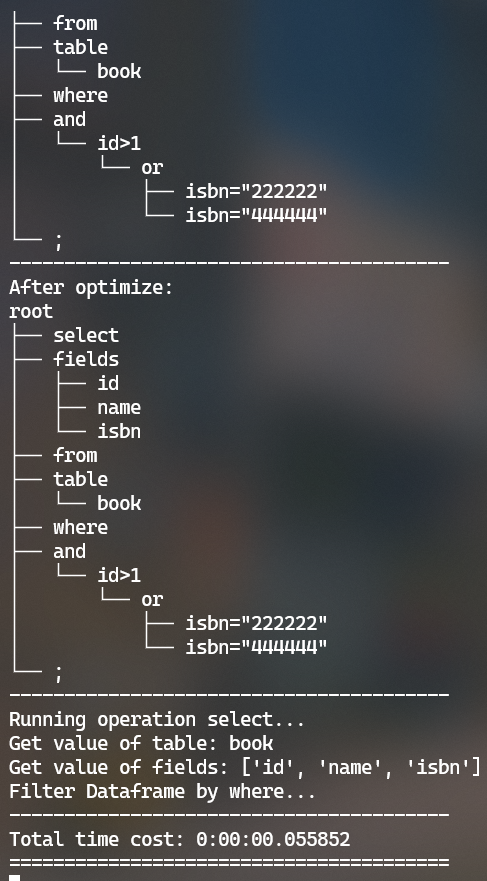
\includegraphics[width=0.475\textwidth]{examples/查询-8002.png}}
    \centering
    \caption{查询数据的屏幕输出}
    \label{fig:select-log}
\end{figure}

图\ref{fig:select-log}展示了查询命令执行后服务端的屏幕输出,可以看出user表的查询命令在8000节点被执行,而book表的查询命令被转发到8002节点执行。另外,嵌套的where子句也按照运算优先级被成功解析成树的形式。

\subsection{删除数据测试}

最后是删除数据的测试,删除数据的sql格式如下:

\begin{lstlisting}
delete from
    <table>
where 
    <condition>;
\end{lstlisting}

\begin{figure}[H]
    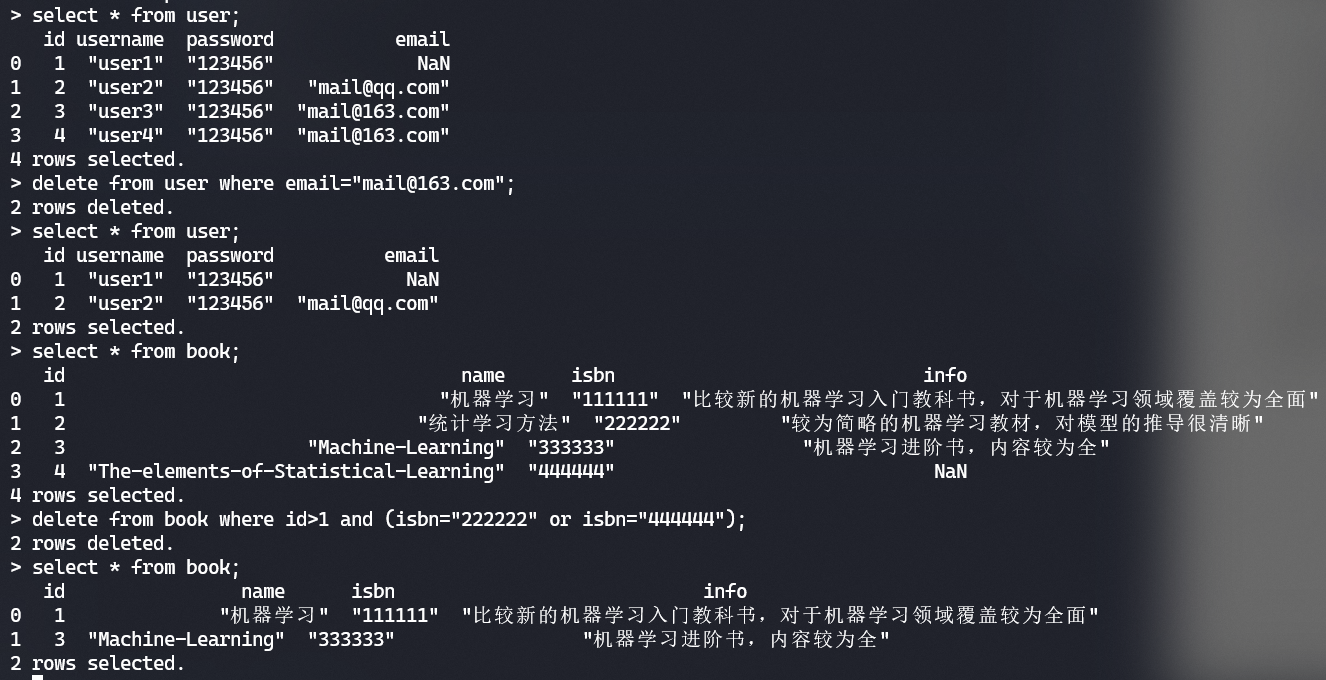
\includegraphics[width=\textwidth]{examples/删除.png}
    \centering
    \caption{删除数据}
    \label{fig:delete}
\end{figure}

图\ref{fig:delete}展示了在客户端输入若干删除数据命令的结果。可以看出,user表中邮箱为"mail@163.com"的记录被成功删除,book表中则是id>1且isbn为"111111"或"333333"的记录被成功删除。

\begin{figure}[H]
    \subfloat[8000节点输出]{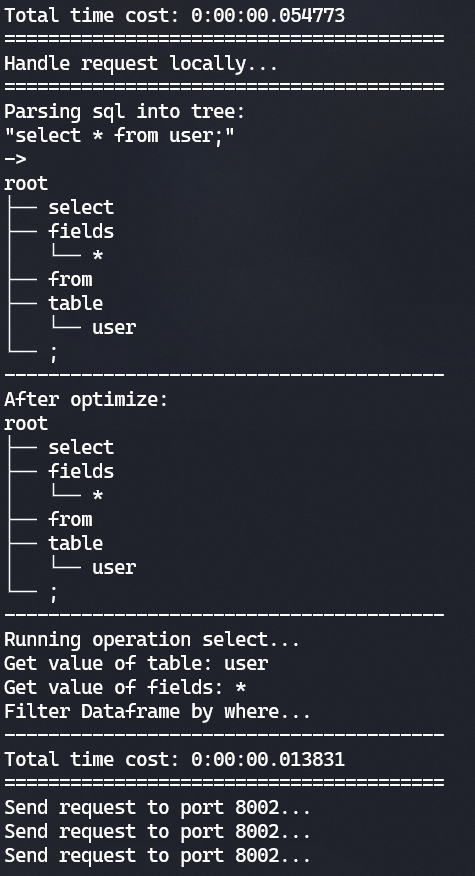
\includegraphics[width=0.34\textwidth]{examples/删除-8000.png}}
    \subfloat[8002节点输出]{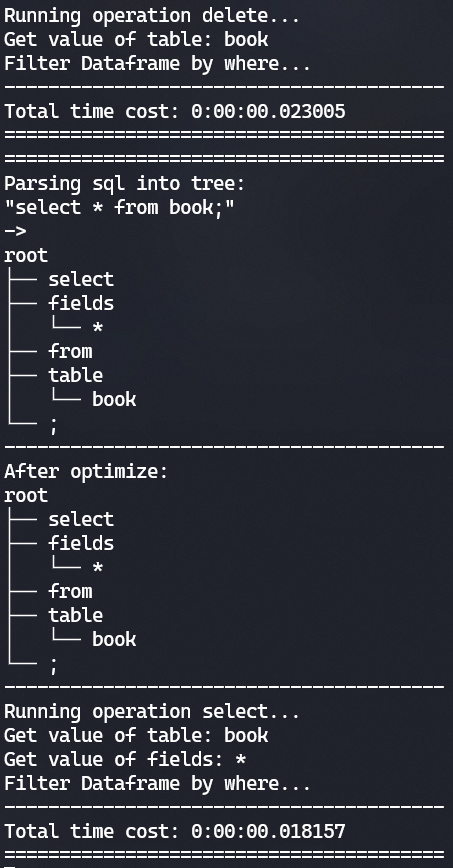
\includegraphics[width=0.325\textwidth]{examples/删除-8002.png}}
    \centering
    \caption{删除数据的屏幕输出}
    \label{fig:delete-log}
\end{figure}

图\ref{fig:delete-log}展示了服务端各节点的屏幕输出,可以看出user表的删除命令在8000节点直接执行,而book表的删除命令被转发到8002节点执行。

\begin{figure}[H]
    \subfloat[]{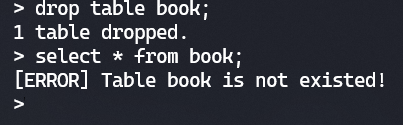
\includegraphics[width=0.7\textwidth]{examples/删除表.png}}
    \subfloat[]{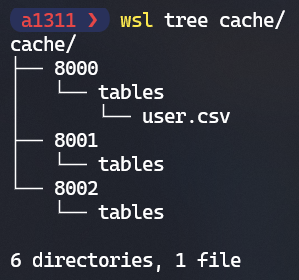
\includegraphics[width=0.3\textwidth]{examples/目录-删除后.png}}
    \centering
    \caption{删除表}
    \label{fig:drop}
\end{figure}

最后,使用drop命令删除book表后,再次使用查询命令。如图\ref{fig:drop}子图(a)所示,将返回"Table book is not existed!"错误。另外,如子图(b)所示,该表在文件系统中已不存在。

至此,本系统的创建表、新增数据、查询数据、删除数据、删除表,以及where子句的解析、数据表的垂直拆分等功能都得以验证,满足实验要求!